\section{Implementação de máquina de café em
VHDL}\label{implementauxe7uxe3o-de-muxe1quina-de-cafuxe9-em-vhdl}

\subsection{Descrição do projeto}\label{descriuxe7uxe3o-do-projeto}

A entidade \texttt{coffee\_machine} recebe uma entrada \texttt{buttons}
de 8 bits procura por duplicatas e gera a saída \texttt{coffee\_out} de
8 bits, que representa as saídas de café. Além disso, há mais uma saída
que representa um error ao processar a entrada, isto é, mais de um ou
nenhum botão pressionado ao mesmo tempo.

\pandocbounded{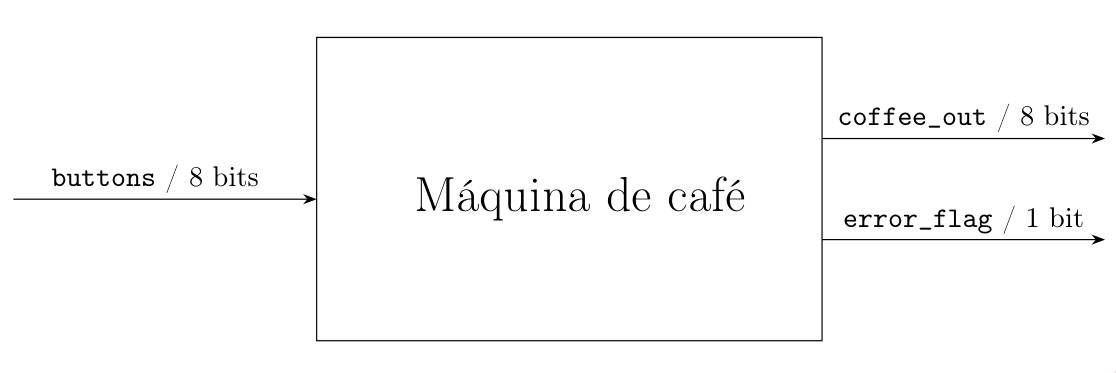
\includegraphics[keepaspectratio]{./assets/diagrama-maquina-de-cafe.png}}

\subsection{Tabela verdade}\label{tabela-verdade}

Seu comportamento é especificado por essa tabela.

\begin{longtable}[]{@{}
  >{\raggedright\arraybackslash}p{(\linewidth - 6\tabcolsep) * \real{0.2277}}
  >{\raggedright\arraybackslash}p{(\linewidth - 6\tabcolsep) * \real{0.2277}}
  >{\raggedright\arraybackslash}p{(\linewidth - 6\tabcolsep) * \real{0.2277}}
  >{\raggedright\arraybackslash}p{(\linewidth - 6\tabcolsep) * \real{0.3168}}@{}}
\toprule\noalign{}
\begin{minipage}[b]{\linewidth}\raggedright
\textbf{Entrada (\texttt{buttons})}
\end{minipage} & \begin{minipage}[b]{\linewidth}\raggedright
\textbf{Saída (\texttt{coffe\_out})}
\end{minipage} & \begin{minipage}[b]{\linewidth}\raggedright
\textbf{Erro (\texttt{error\_flag})}
\end{minipage} & \begin{minipage}[b]{\linewidth}\raggedright
\textbf{Descrição}
\end{minipage} \\
\midrule\noalign{}
\endhead
\bottomrule\noalign{}
\endlastfoot
\texttt{0000\ 0000} & \texttt{0000\ 0000} & \texttt{1} & Nenhum botão
pressionado (erro). \\
\texttt{0000\ 0001} & \texttt{0000\ 0001} & \texttt{0} & Botão 0
pressionado. Café 0. \\
\texttt{0000\ 0010} & \texttt{0000\ 0010} & \texttt{0} & Botão 1
pressionado. Café 1. \\
\texttt{0000\ 0100} & \texttt{0000\ 0100} & \texttt{0} & Botão 2
pressionado. Café 2. \\
\texttt{0000\ 1000} & \texttt{0000\ 1000} & \texttt{0} & Botão 3
pressionado. Café 3. \\
\texttt{0001\ 0000} & \texttt{0001\ 0000} & \texttt{0} & Botão 4
pressionado. Café 4. \\
\texttt{0010\ 0000} & \texttt{0010\ 0000} & \texttt{0} & Botão 5
pressionado. Café 5. \\
\texttt{0100\ 0000} & \texttt{0100\ 0000} & \texttt{0} & Botão 6
pressionado. Café 6. \\
\texttt{1000\ 0000} & \texttt{1000\ 0000} & \texttt{0} & Botão 7
pressionado. Café 7. \\
\texttt{XXXX\ XXXX} & \texttt{0000\ 0000} & \texttt{1} & Qualquer outra
entrada (erro). \\
\end{longtable}

\subsection{Plano de simulação e
Simulação}\label{plano-de-simulauxe7uxe3o-e-simulauxe7uxe3o}

Para assertar o funcionamento da nossa implementação, vamos testar as
seguintes entradas:

\subsubsection{\texorpdfstring{Cenários de Teste para a Entidade
\texttt{coffe\_machine}}{Cenários de Teste para a Entidade coffe\_machine}}\label{cenuxe1rios-de-teste-para-a-entidade-coffe_machine}

\begin{longtable}[]{@{}
  >{\raggedright\arraybackslash}p{(\linewidth - 8\tabcolsep) * \real{0.1197}}
  >{\raggedright\arraybackslash}p{(\linewidth - 8\tabcolsep) * \real{0.1620}}
  >{\raggedright\arraybackslash}p{(\linewidth - 8\tabcolsep) * \real{0.2254}}
  >{\raggedright\arraybackslash}p{(\linewidth - 8\tabcolsep) * \real{0.1620}}
  >{\raggedright\arraybackslash}p{(\linewidth - 8\tabcolsep) * \real{0.3310}}@{}}
\toprule\noalign{}
\begin{minipage}[b]{\linewidth}\raggedright
\textbf{Caso de Teste}
\end{minipage} & \begin{minipage}[b]{\linewidth}\raggedright
\textbf{Entrada (\texttt{buttons})}
\end{minipage} & \begin{minipage}[b]{\linewidth}\raggedright
\textbf{Saída Esperada (\texttt{coffe\_out})}
\end{minipage} & \begin{minipage}[b]{\linewidth}\raggedright
\textbf{Erro (\texttt{error\_flag})}
\end{minipage} & \begin{minipage}[b]{\linewidth}\raggedright
\textbf{Descrição}
\end{minipage} \\
\midrule\noalign{}
\endhead
\bottomrule\noalign{}
\endlastfoot
\textbf{Teste 1} & \texttt{0000\ 0100} & \texttt{0000\ 0100} &
\texttt{0} & Apenas o botão 2 foi pressionado. Café 2. \\
\textbf{Teste 2} & \texttt{1000\ 0000} & \texttt{1000\ 0000} &
\texttt{0} & Apenas o botão 7 foi pressionado. Café 7. \\
\textbf{Teste 3} & \texttt{0000\ 0000} & \texttt{0000\ 0000} &
\texttt{1} & Nenhum botão foi pressionado. Erro. \\
\textbf{Teste 4} & \texttt{0000\ 1110} & \texttt{0000\ 0000} &
\texttt{1} & Mais de um botão pressionado (botões 1, 2 e 3). \\
\end{longtable}
